% This file was created with tikzplotlib v0.10.1.
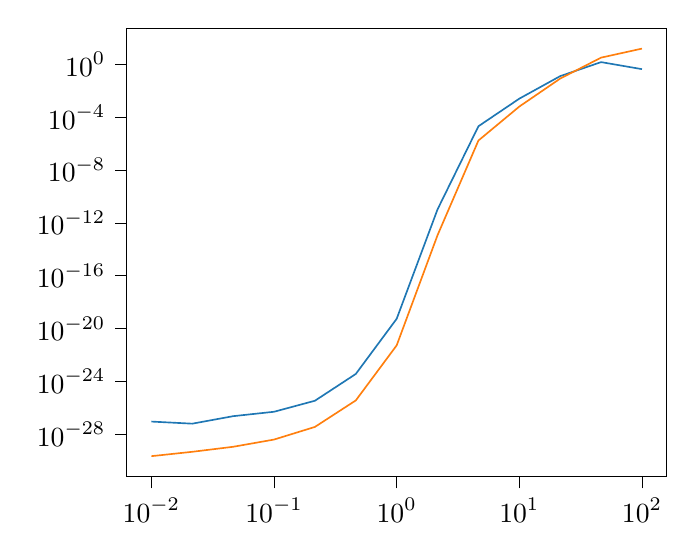
\begin{tikzpicture}

\definecolor{darkgray176}{RGB}{176,176,176}
\definecolor{darkorange25512714}{RGB}{255,127,14}
\definecolor{steelblue31119180}{RGB}{31,119,180}

\begin{axis}[
log basis x={10},
log basis y={10},
tick align=outside,
tick pos=left,
x grid style={darkgray176},
xmin=0.00630957329672048, xmax=158.489319423237,
xmode=log,
xtick style={color=black},
xtick={0.0001,0.001,0.01,0.1,1,10,100,1000,10000},
xticklabels={
  \(\displaystyle {10^{-4}}\),
  \(\displaystyle {10^{-3}}\),
  \(\displaystyle {10^{-2}}\),
  \(\displaystyle {10^{-1}}\),
  \(\displaystyle {10^{0}}\),
  \(\displaystyle {10^{1}}\),
  \(\displaystyle {10^{2}}\),
  \(\displaystyle {10^{3}}\),
  \(\displaystyle {10^{4}}\)
},
y grid style={darkgray176},
ymin=6.35347696969342e-32, ymax=528.901981965432,
ymode=log,
ytick style={color=black},
ytick={1e-36,1e-32,1e-28,1e-24,1e-20,1e-16,1e-12,1e-08,0.0001,1,10000,100000000},
yticklabels={
  \(\displaystyle {10^{-36}}\),
  \(\displaystyle {10^{-32}}\),
  \(\displaystyle {10^{-28}}\),
  \(\displaystyle {10^{-24}}\),
  \(\displaystyle {10^{-20}}\),
  \(\displaystyle {10^{-16}}\),
  \(\displaystyle {10^{-12}}\),
  \(\displaystyle {10^{-8}}\),
  \(\displaystyle {10^{-4}}\),
  \(\displaystyle {10^{0}}\),
  \(\displaystyle {10^{4}}\),
  \(\displaystyle {10^{8}}\)
}
]
\addplot [semithick, steelblue31119180]
table {%
0.00999999977648258 9.1700004612442e-28
0.0215443465858698 6.35496644266094e-28
0.046415887773037 2.34883279675772e-27
0.100000001490116 5.06391451090609e-27
0.215443462133408 3.45279394495563e-26
0.464158892631531 3.6685827446471e-24
1 5.48088886437308e-20
2.15443468093872 1.04830852946436e-11
4.64158868789673 2.02942080131244e-05
10 0.00248512436412089
21.5443477630615 0.125801816392909
46.4158897399902 1.44396219040218
100 0.423086200181043
};
\addplot [semithick, darkorange25512714]
table {%
0.00999999977648258 2.21231098209957e-30
0.0215443465858698 4.72972723377982e-30
0.046415887773037 1.13426533598971e-29
0.100000001490116 3.99196992983243e-29
0.215443462133408 3.60685542411464e-28
0.464158892631531 3.64750783836672e-26
1 5.34916456919715e-22
2.15443468093872 1.16618567633735e-13
4.64158868789673 1.69273401963915e-06
10 0.000627079343827502
21.5443477630615 0.0820572523687714
46.4158897399902 3.15287810504374
100 15.1893951114118
};
\end{axis}

\end{tikzpicture}
